\documentclass[UTF8]{ctexart}
\usepackage[margin=1in]{geometry}
\usepackage{amsmath}
\usepackage{amssymb}
\usepackage{listings}
\usepackage{xcolor}
\usepackage{graphicx}
\usepackage{hyperref}
\usepackage{algorithmic}
\usepackage{algorithm}
\usepackage{tikz}
\usetikzlibrary{arrows.meta,positioning}

% 代码格式设置
\lstset{
    language=C++,
    basicstyle=\ttfamily\small,
    breaklines=true,
    numbers=left,
    numberstyle=\tiny,
    keywordstyle=\color{blue},
    commentstyle=\color{gray},
    stringstyle=\color{red},
    showstringspaces=false,
    backgroundcolor=\color{lightgray!20},
    frame=single
}

\title{\textbf{堆排序 (Heap Sort)}}
\author{}
\date{}

\begin{document}

\maketitle

\section{堆的定义}

\subsection{什么是堆(Heap)?}

堆是一种特殊的二叉树数据结构,满足以下特性:

\textbf{最大堆(Max-Heap):}树中任意节点的值至少与其子节点的值一样大。即对于任意节点,有 $\text{parent} \geq \text{left\_child}$ 且 $\text{parent} \geq \text{right\_child}$。

\textbf{最小堆(Min-Heap):}树中任意节点的值至多与其子节点的值一样大。即对于任意节点,有 $\text{parent} \leq \text{left\_child}$ 且 $\text{parent} \leq \text{right\_child}$。

\textbf{堆的性质:}
\begin{itemize}
    \item 根节点包含最大值(最大堆)或最小值(最小堆)
    \item 堆是完全二叉树,即除最后一层外,所有层都已填满,最后一层从左向右填充
    \item 高度为 $\log_2(n)$,其中 $n$ 是节点数
\end{itemize}

\section{堆的数组表示}

\subsection{数组索引与树结构的对应关系}

对于以数组 $A$ 存储的堆,编号从1开始:

\begin{itemize}
    \item 节点 $i$ 的值存储在 $A[i]$
    \item 节点 $i$ 的左子节点:$A[2i]$
    \item 节点 $i$ 的右子节点:$A[2i+1]$
    \item 节点 $j$ 的父节点:$A[\lfloor j/2 \rfloor]$
    \item 所有叶子节点的编号范围:$\lfloor n/2 \rfloor + 1$ 到 $n$
\end{itemize}

\textbf{示例:}数组 $[12, 10, 6, 5, 4, 3]$ 表示的堆结构:

\begin{center}
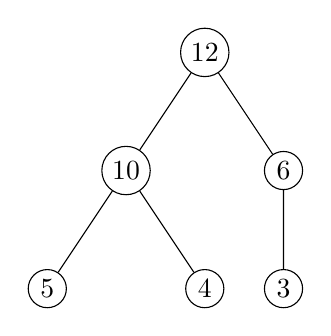
\begin{tikzpicture}[level distance=15mm, sibling distance=20mm, every node/.style={circle,draw,inner sep=2pt}]
\node {12}
  child { node {10}
    child { node {5} }
    child { node {4} }
  }
  child { node {6}
    child { node {3} }
  };
\end{tikzpicture}
\end{center}

\section{Heapify操作}

\subsection{堆调整(Heapify)的定义与实现}

当堆的根节点被移除后,需要从新的根节点开始,通过"向下推"操作来恢复堆的性质。具体步骤:

\begin{enumerate}
    \item 取出叶子节点作为新的根
    \item 将该节点与其最大的子节点进行比较
    \item 如果违反堆的性质,交换两者
    \item 继续向下比较和交换,直到堆的性质恢复
\end{enumerate}

\subsubsection{Heapify伪代码(见第3页)}

\begin{algorithm}
\caption{Heapify操作伪代码}
\begin{algorithmic}
\STATE \textbf{procedure} Heapify(A, i, n)
\COMMENT{维护以 A[i] 为根的子堆的堆性质,堆的大小为 n}
\STATE r $\leftarrow$ i
\WHILE{r $\leq$ $\lfloor n/2 \rfloor$}  \COMMENT{r 有子节点}
    \IF{2r == n}  \COMMENT{r 只有一个左子节点}
        \IF{A[r] < A[2r]}
            \STATE swap(A[r], A[2r])
            \STATE \textbf{break}
        \ENDIF
    \ELSE  \COMMENT{r 有两个子节点}
        \IF{(A[r] < A[2r]) \AND (A[2r] > A[2r+1])}
            \STATE swap(A[r], A[2r])
            \STATE r $\leftarrow$ 2r
        \ELSIF{(A[r] < A[2r+1]) \AND (A[2r+1] > A[2r])}
            \STATE swap(A[r], A[2r+1])
            \STATE r $\leftarrow$ 2r + 1
        \ELSE
            \STATE \textbf{break}  \COMMENT{已满足堆性质}
        \ENDIF
    \ENDIF
\ENDWHILE
\STATE \textbf{end procedure}
\end{algorithmic}
\end{algorithm}

\subsubsection{时间复杂度}

\textbf{时间复杂度:}$O(h)$,其中 $h$ 是堆的高度,$h = \log_2(n)$

\section{构建堆}

\subsection{BuildHeap操作}

从一个无序数组构建堆的方法是逐个对非叶子节点执行 Heapify 操作:

\begin{algorithm}
\caption{构建堆伪代码}
\begin{algorithmic}
\STATE \textbf{procedure} BuildHeap(A)
\STATE n $\leftarrow$ length of A
\FOR{i = $\lfloor n/2 \rfloor$ \textbf{downto} 1}
    \STATE Heapify(A, i, n)
\ENDFOR
\STATE \textbf{end procedure}
\end{algorithmic}
\end{algorithm}

\textbf{关键观察:}
\begin{itemize}
    \item 最后一个节点为 $A[n]$,其父节点为 $A[\lfloor n/2 \rfloor]$
    \item 因此,所有叶子节点 $A[\lfloor n/2 \rfloor + 1], \ldots, A[n]$ 已经满足堆性质,无需处理
    \item 只需从 $\lfloor n/2 \rfloor$ 向下处理到 1
\end{itemize}

\subsection{BuildHeap的复杂度分析}

对于高度为 $h = \log_2(n)$ 的堆,节点的分布如下:

\begin{itemize}
    \item 高度 $h$ 的节点:最多 1 个,Heapify 耗时 $O(h)$
    \item 高度 $h-1$ 的节点:最多 2 个,Heapify 耗时 $O(h-1)$
    \item 高度 $h-2$ 的节点:最多 4 个,Heapify 耗时 $O(h-2)$
    \item $\vdots$
    \item 高度 0 的节点:最多 $2^h$ 个(在构建中被跳过)
\end{itemize}

BuildHeap 的总复杂度:

\begin{equation}
O\left(\sum_{i=1}^{h} i \cdot 2^{h-i}\right) = O(2^h) = O(n)
\end{equation}

\textbf{结论:}虽然单次 Heapify 耗时 $O(\log n)$,但构建整个堆的时间复杂度仅为 $O(n)$。

\section{堆排序算法}

\subsection{基本思想}

堆排序利用堆的特性来高效地找到最大元素:

\begin{enumerate}
    \item 将无序数组构建成最大堆
    \item 重复以下步骤:
    \begin{itemize}
        \item 将堆的根节点(最大元素)与最后一个元素交换
        \item 减少堆的大小
        \item 对新的根节点执行 Heapify 以恢复堆性质
    \end{itemize}
    \item 直到堆的大小减为 1
\end{enumerate}

\subsection{堆排序伪代码}

\begin{algorithm}
\caption{堆排序伪代码}
\begin{algorithmic}
\STATE \textbf{procedure} HeapSort(A)
\STATE n $\leftarrow$ length of A
\STATE BuildHeap(A)  \COMMENT{第一步:构建最大堆}
\FOR{i = n \textbf{downto} 2}
    \STATE swap(A[1], A[i])  \COMMENT{将最大元素移到末尾}
    \STATE Heapify(A, 1, i-1)  \COMMENT{对缩小的堆进行调整}
\ENDFOR
\STATE \textbf{end procedure}
\end{algorithmic}
\end{algorithm}

\subsection{时间复杂度分析}

\begin{itemize}
    \item BuildHeap 的复杂度:$O(n)$
    \item 主循环执行 $n-1$ 次,每次 Heapify 耗时 $O(\log n)$
    \item 总体复杂度:$O(n) + (n-1) \times O(\log n) = O(n \log n)$
\end{itemize}

\textbf{最坏、平均、最好情况的时间复杂度均为 $O(n \log n)$。}

\subsection{空间和稳定性}

\begin{itemize}
    \item \textbf{空间复杂度:}$O(1)$(原地排序)
    \item \textbf{稳定性:}不稳定(相等元素的相对顺序可能改变)
\end{itemize}

\section{优先队列应用}

\subsection{优先队列的定义}

优先队列是一种抽象数据类型,支持以下三种操作:

\begin{itemize}
    \item \textbf{INSERT(S, x):}将元素 $x$ 插入集合 $S$
    \item \textbf{MAXIMUM(S):}返回 $S$ 中的最大元素
    \item \textbf{DELETE\_MAX(S):}移除并返回 $S$ 中的最大元素
\end{itemize}

\textbf{应用场景:}
\begin{itemize}
    \item 操作系统中的进程调度
    \item 网络中的数据包管理
    \item 医院挂号系统中的患者优先级管理
    \item Dijkstra 算法和 Prim 算法中的顶点选择
\end{itemize}

\subsection{使用堆实现优先队列}

\subsubsection{MAXIMUM操作}

\begin{algorithm}
\caption{获取最大元素}
\begin{algorithmic}
\STATE \textbf{function} MAXIMUM(S)
\COMMENT{假设元素存储在堆 A 中}
\STATE \textbf{return} A[1]  \COMMENT{最大值总在根节点}
\STATE \textbf{end function}
\end{algorithmic}
\end{algorithm}

时间复杂度:$O(1)$

\subsubsection{DELETE\_MAX操作}

\begin{algorithm}
\caption{删除最大元素}
\begin{algorithmic}
\STATE \textbf{procedure} DELETE\_MAX(S)
\IF{n < 1}
    \STATE \textbf{return} ``Heap underflow''
\ENDIF
\STATE swap(A[1], A[n])  \COMMENT{将最后一个元素移到根}
\STATE n $\leftarrow$ n - 1  \COMMENT{减少堆的大小}
\STATE Heapify(A, 1, n)  \COMMENT{恢复堆性质}
\STATE \textbf{end procedure}
\end{algorithmic}
\end{algorithm}

时间复杂度:$O(\log n)$

\subsubsection{INSERT操作}

插入操作与 Heapify 相反,通过"向上推"来恢复堆性质:

\begin{algorithm}
\caption{插入元素}
\begin{algorithmic}
\STATE \textbf{procedure} INSERT(S, x)
\STATE n $\leftarrow$ n + 1
\STATE A[n] $\leftarrow$ x  \COMMENT{将新元素添加到末尾}
\STATE i $\leftarrow$ n
\WHILE{(i > 1) \AND (A[\lfloor i/2 \rfloor] < A[i])}
    \STATE swap(A[i], A[\lfloor i/2 \rfloor])  \COMMENT{与父节点交换}
    \STATE i $\leftarrow$ \lfloor i/2 \rfloor  \COMMENT{向上移动}
\ENDWHILE
\STATE \textbf{end procedure}
\end{algorithmic}
\end{algorithm}

时间复杂度:$O(\log n)$

\section{算法总结}

\subsection{堆排序的优缺点}

\textbf{优点:}

\begin{itemize}
    \item 时间复杂度为 $O(n \log n)$,对于大规模数据高效
    \item 原地排序,空间复杂度只有 $O(1)$
    \item 不依赖输入数据的初始顺序,性能稳定
    \item 堆的实现可用于优先队列等多种应用
\end{itemize}

\textbf{缺点:}

\begin{itemize}
    \item 不是稳定排序
    \item 实际应用中常数因子较大,不如快速排序快
    \item 对于已排序或部分排序的数据也需要 $O(n \log n)$ 时间(不自适应)
\end{itemize}

\subsection{与其他排序算法的比较}

\begin{table}[h]
\centering
\begin{tabular}{|c|c|c|c|}
\hline
\textbf{算法} & \textbf{时间复杂度} & \textbf{空间复杂度} & \textbf{稳定性} \\
\hline
选择排序 & $O(n^2)$ & $O(1)$ & 否 \\
\hline
冒泡排序 & $O(n^2)$ & $O(1)$ & 是 \\
\hline
插入排序 & $O(n^2)$ & $O(1)$ & 是 \\
\hline
堆排序 & $O(n \log n)$ & $O(1)$ & 否 \\
\hline
快速排序 & $O(n \log n)$ & $O(\log n)$ & 否 \\
\hline
归并排序 & $O(n \log n)$ & $O(n)$ & 是 \\
\hline
\end{tabular}
\end{table}

\end{document}
